%ot-term-paper.tex
\documentclass[12pt]{article}
\usepackage{amssymb,latexsym}
\usepackage[round,sort]{natbib}
\usepackage{fancyhdr}
\usepackage{lastpage}
\usepackage{graphicx}
\graphicspath{ {ot-term-paper-images/} }
\usepackage[T1]{fontenc}
\usepackage{mathptmx}
\usepackage{tabu}
\usepackage{textcomp}
\usepackage{listings}
\usepackage[a4paper]{geometry}
\usepackage{hyperref}
\usepackage{tabu}
\hypersetup{
    colorlinks=true,
    linkcolor=blue,
    filecolor=magenta,      
    urlcolor=cyan,
    citecolor=magenta,
}
\geometry{
 total={150mm,247mm},
 left=25mm,
 top=25mm,
}
\lstset{
basicstyle=\ttfamily,
columns=flexible,
breaklines=true
}
\newenvironment{hypothesis}{
  	\itshape
  	\leftskip=\parindent \rightskip=\parindent
  	\noindent\ignorespaces}
	
\pagestyle{fancy}
\fancyhf{}
\lhead{Embedded agency in institutional fields}
\rfoot{Page \thepage  \ of \pageref{LastPage}}
\rhead{Iyenggar}

\begin{document}
\title{Embedded Agency in Institutional Fields:\\  Developing Theory From a Matching Game}
\author{Ashwin Iyenggar  (1521001) \\ ashwin.iyenggar15@iimb.ernet.in} 

\maketitle

\begin{abstract}
We apply a formal model to understand the effects of initial orientations and learning rates on the outcomes in an institutional context. We find that the relative rates of learning of the institutional field and the embedded agent influence overall performance outcomes in a matching game. We contribute to the theory on the role and effects of embedded agency in institutional fields with a nuanced set of hypotheses backed by a formal model.
\end{abstract}


{Keywords:} Embedded Agency, Institutional Fields, Agent Based Models, Matching Game, Reinforcement Learning

\section{Introduction}\label{S:Introduction}
Our understanding of  institutionalization has come a long way since \cite{Selznick1957} made the startling observation that organizations adopted new goals suited to existing structures  instead of changing the structures that may have outlived their utility. Several years later, the misinterpretation of the "iron cage" metaphor from  \cite{Dimaggio1983} had precipitated the introduction of the notion of agency in the form of institutional entrepreneurship in \cite{Dimaggio1988}. Since then, institutional theorists have grappled with understanding the interplay between  actors within the organizational field and the organizational field itself.  \cite{Selznick1996} suggested that the formal structure should be ideally seen as an adaptive product, responsive to environmental influences, including cultural definitions of propriety and legitimacy. Our point of view is well captured by \cite{Philips2009} who suggest that institutional entrepreneurship is an important idea because it considers how actors can attain their goals by intentionally constructing and/or altering the institutional structures in which they are embedded. \\\\

\noindent Despite scholars calling attention to the value of understanding the agent-field dynamic, a rigorously developed, nuanced understanding of embedded agency has seemed elusive. Indeed the role of agency seems to have been carried too far. This is captured by \cite{Suddaby2010} who suggests that research in institutional theory is plagued with the problem of organizations now being presented as "hypermuscular supermen" instead of the "passive cultural dopes" earlier. Clearly, there is a need for more integrative institutional theory that can inform how organizations operating in their respective institutional fields straddle this continuum between the characterizations of "hypermuscular supermen" on the one extreme (suggesting high levels of agency) and that of "passive cultural dopes" (suggesting high levels of structuration of the institutional fields).\\\\

\noindent We attempt to contribute to this conversation by generating hypotheses developed from a formal model of agent-field learning and interaction. While it must be acknowledged up front that formal and computational models are at best an aid to developing theory, a few points deserve attention. First, by allowing the researcher the flexibility to control the variables that change, computational models provide the researcher with focussed and crisp hypotheses concerning specific aspects of the phenomenon under study. Second, formal models allow for easier comparison between competing models, and for theory building in the process. Finally, computational models allow for more complex models to be built on top of earlier models, thus aggregating the knowledge base in an area over time. That said, such a method of theory generation is no substitute for empirical research. Formal and computational models and empirical research seem more complementary, with the former being an aid to developing theory while the latter being a tool to test theory. However, the objective of this article is to use a formal computational model to generate hypotheses that may inform further empirical work. Any empirical work however will remain outside the scope of this article.\\\\

\noindent In this article, we apply a simple matching game model to  understand the dynamics of the interaction between embedded agents and the institutional field. Despite the simplicity of the model (it models the institutional field and the embedded agent as two players), our model provides us with the opportunity to propose hypotheses that would be difficult to easily explicate cleanly in a typical empirical setting.\\\\

\noindent The rest of this article is organized as follows. In the following section, we summarize the key constructs and definitions in institutional theory that we build upon in this article. We then present the assumptions and the formal definitions for the model. A subset of our initial results from the computer simulations of the model are then presented in the following section. We propose hypotheses on the dynamics of embedded agency and their institutional fields based on our findings from our computer simulation. We conclude with a call for continuing this path for theory development, and for empirical studies to use the theoretical frames developed here for understanding empirical validity of the hypotheses proposed.\\\\

\section{Background}
Before proceeding with the model, we discuss here some of the salient constructs within institutional theory so as to be on the same page in the discussions later in the article. \cite{Scott1995} visualized institutional fields as a community of organizations that partakes of a common meaning system and whose participants interact more frequently and fatefully with one another than with actors outside the field. This definition was on lines similar to that of \cite{Dimaggio1983} who defined organizational fields as those organizations that in the aggregate constitute a recognized area of institutional life: key suppliers, resource and product consumers, regulatory agencies, and other organizations that produce similar services or products. \\\\
Scholars have suggested that legitimacy is an important aspect of the institutional setup and that it  is achieved primarily through isomorphism \citep{Kostova2008}, where organizations become similar to other organizations in their organizational field. However, little seems to have been understood about the processes of legitimation \citep{Harmon2015}. \\\\
On the other hand, organizations seem to engage in ceremonial adoption of institutionalized structures and practices while at the same time decoupling themselves from the environment by actually using different structures and practices they view as more economically efficient \citep{Kostova2008}. Recent rhetorical theory has emphasized the role of audience in affecting the way rhetoric shapes social action. Finally, the paradox of embedded agency refers  to the following tension: how can organizations or individuals innovate if their beliefs and actions are determined by the institutional environment they wish to change \citep{Scott1987}? \\\\
A common thread across the arguments for legitimacy, decoupling, rhetoric and the paradox is that the mechanism that explains the agent-field dynamic is not clear. Our work in this article is addressed toward this gap in our collective theoretical understanding. Specifically, we model heterogeniety in the relative learning rates of the agent and the field in the presence frequent interaction as a plausible mechanism driving the agent-field relationship.

\section{Model}

We develop a simple model consisting of two players who participate in a repeated game of matching\footnote{I am grateful to Phanish Puranam for having introduced me to this model of reinforcement learning during a workshop at the Indian Institute of Science on 16th December, 2016. His definitions and code have been extensively reused in this work.}. Our study will assume the two players to be the institutional field (F), and the embedded agent (A). In each time period each of the players can make one of two decision choices 0 or 1. At the start of the game, the institutional field F choses choice 0 with probability $p_{0,F}^0$ and choice 1 with probability $1 - p_{0,F}^0$. Similarly, at the start of the game, the agent A choses choice 0 with probability $p_{0,A}^0$ and choice 1 with probability $1 - p_{0,A}^0$. When the choices of the field F and agent A match in a time period, they each get a payoff of 1 in that period. Otherwise they each get a payoff of 0. The payoffs are captured by the matrix in Table ~\ref{payoffmatrix}\\\\

\begin{table}
\begin{centering}
\caption {Payoff Matrix}
\label{payoffmatrix}
{\tabulinesep=1.4mm
\begin{tabu}{|c|c|c|}
\hline
&$choice_F(t) = 0$&$choice_F(t) = 1$\\\hline
$choice_A(t) = 0$&$[payoff_F(t),payoff_A(t)]=[1,1]$&$[payoff_F(t),payoff_A(t)]=[0,0]$\\\hline
$choice_A(t) = 1$&$[payoff_F(t),payoff_A(t)]=[0,0]$&$[payoff_F(t),payoff_A(t)]=[1,1]$\\\hline
\end{tabu}}

\end{centering}
\end{table} 


\noindent At the end of round t, both the field F and the agent A update their respective probabilities $p_{t+1,F}^0$ and $p_{t+1,A}^0$ based on their prior probabilities ($p_{t,F}^0$ and $p_{t,A}^0$) and their respective learning rates $\phi_F$ and $\phi_A$. We expect the field F and agent A to update their prior probabilities along the lines of the theory on reinforcement learning. We define $\phi$ as the learning rate function that make take any value between 0 and 1. A $\phi$ value of 0 indicates no learning, while a $\phi$ value of 1 indicates perfect learning.  Agents update their prior probabilities based on their respective learning rates $\phi_F$ and $\phi_A$ respectively. The rules used to update prior probabilities are laid out in the matrix in Table ~\ref{priorsupdation}.\\\\\
\begin{table}
\begin{centering}
\caption {Matrix of Rules for Updating Prior Probabilities}
\label{priorsupdation}
\medskip
{\tabulinesep=1.4mm
\begin{tabu}{|c|c|c|}
\hline
&$payoff(t) = 1$&$payoff(t) = 0$\\\hline
$choice(t) = 0$&$p_{t+1}^0=p_t^0+\phi(1-p_t^0)$&$p_{t+1}^0=p_t^0-\phi(p_t^0)$\\\hline
$choice(t) = 1$&$p_{t+1}^0=p_t^0-\phi(p_t^0)$&$p_{t+1}^0=p_t^0+\phi(1-p_t^0)$\\\hline
\end{tabu}}
\medskip

\end{centering}
\end{table}

\noindent An intuitive way of thinking about our assumptions are that both players win when they are aligned on the decision. The specific configuration of the alignment does not impact the payoffs beyond their being the same. Therefore (0,0) would be just as good an outcome as (1,1). The intuition behind the updating of prior probabilities in ~\ref{priorsupdation} is that both agents and the institutional fields learn to understand the other's preferences over multiple interactions based on their inherent learning rates. Since the payoffs exist only when there is agreement on the outcome, we would expect that either player would, at their given rate of learning try to adjust to the other.\\\\
 
\noindent For the purposes of this paper, we assume that the rates of learning $\phi_F$ and $\phi_A$ remain constant for entire duration of the game\footnote{While outside the scope of the current article, it seems reasonable that boundedly rational agents could also update their rates of learning in response to the payoffs. It would be an interesting extension of the current work to consider the impact of making this assumption}. However, the application of the learning rate to prior probabilities opens the opportunity for the respective probabilities $p_F$ and $p_A$ to change from one time period to another. The above was coded in a Python program and analyzed using Stata, the code for both of which have been shared in the appendix.\\\\
Before proceeding to interpret the results of the simulations, some terms need to be introduced and defined. From the prior sections, we understand the prior probabilities $p_{t,F}^0$ and $p_{t,A}^0$ as the probability with which the field F and the agent A will choose the outcome 0 in time period $t$. We understand that these probabilities are computed for each time period after taking into account both the choice made in the previous period, and the learning rate $\phi$ defined for each of F and A. \\\\
In  order to make our analysis a little more intuitive, we further define a few categories. For the learning rate $\phi$, we define three categories: Slow ($\phi <= 0.05$), Medium ($0.05 < \phi <= 0.3$) and Fast  ($0.3 < \phi <= 0.7$). In the models to follow, we additionally assume that agents may have learning rates of Slow, Medium and Fast, while Fields may have learning rates of Slow and Medium. Since $choice(t)$ is either 0 or 1 for each player, with 0 being picked with a probability of $p_{t,F}^0$ by the field F and 0 being picked with a probability of $p_{t,A}^0$ by the agent A. In order to make it easier to communicate categories, we use the following definitions while referring to prior probabilities of player choice. \\\\
\textbf{Field Start Position}\\\\
We define $0 <= p_{0,F}^0 <= 0.1$ as being Left (L),  $0.1 < p_{0,F}^0 <= 0.35$ as Left of Center (LC), $0.35 < p_{0,F}^0 <= 0.65$ as Center (C),  $0.65 < p_{0,F}^0 < 0.9$ as  Right of Center (RC), and $0.9 <= p_{0,F}^0 <= 1$ as Right (R). For the analysis in this article however, we restrict ourselves to only two of the five Field Start Positions, viz: Right of Center (RC) and Right (R)\\\\
\textbf{Agent Start Position}\\\\
We define three categories for the Agent Start Position, as a function dependent on the starting prior probability of the agent relative to the starting prior probability of the field. First, the agent start position is said to be \textbf{Aligned} if $p_{0,A}^0 = 0.95$, to be \textbf{Agnostic} if $p_{0,A}^0 = 0.5$ and to be \textbf{Adversarial} if $p_{0,A}^0 = 0.05$. \textbf{Aligned} suggests that both the field F and the agent A have a higher starting prior probability of picking 0 (Note from the previous section that under configurations R and RC that we have restricted our experiments to, field F is more likely to pick 0 in all conditions). \textbf{Adversarial} suggests that the field F and the agent A have opposite orientations toward picking 0 as the outcome at the start (i.e., this would mean $p_{0,A}^0 = 0.05$ for both R and RC configurations of the field F). \textbf{Agnostic} suggests that the agent A starts off without preferring outcome 0 over outcome 1, therefore with $p_{0,A}^0 = 0.5$.\\\\

\noindent The prior probabilities of the field F (captured by R, or RC), of the agent A (captured by Aligned, Agnostic, or Adversarial) and the relative rates of learning (Slow, Medium, Fast) are the mechanisms that we model to demonstrate the dynamic in the interaction between the embedded agent and the institutional field. The following section discusses the results of the simulation experiments that were run on 1000 pairs of agents over 100 periods. While we ran experiments on 54 unique configurations, we discuss only a fraction of them in this article.\\\\
\begin{figure}[h]
\begin{centering}
  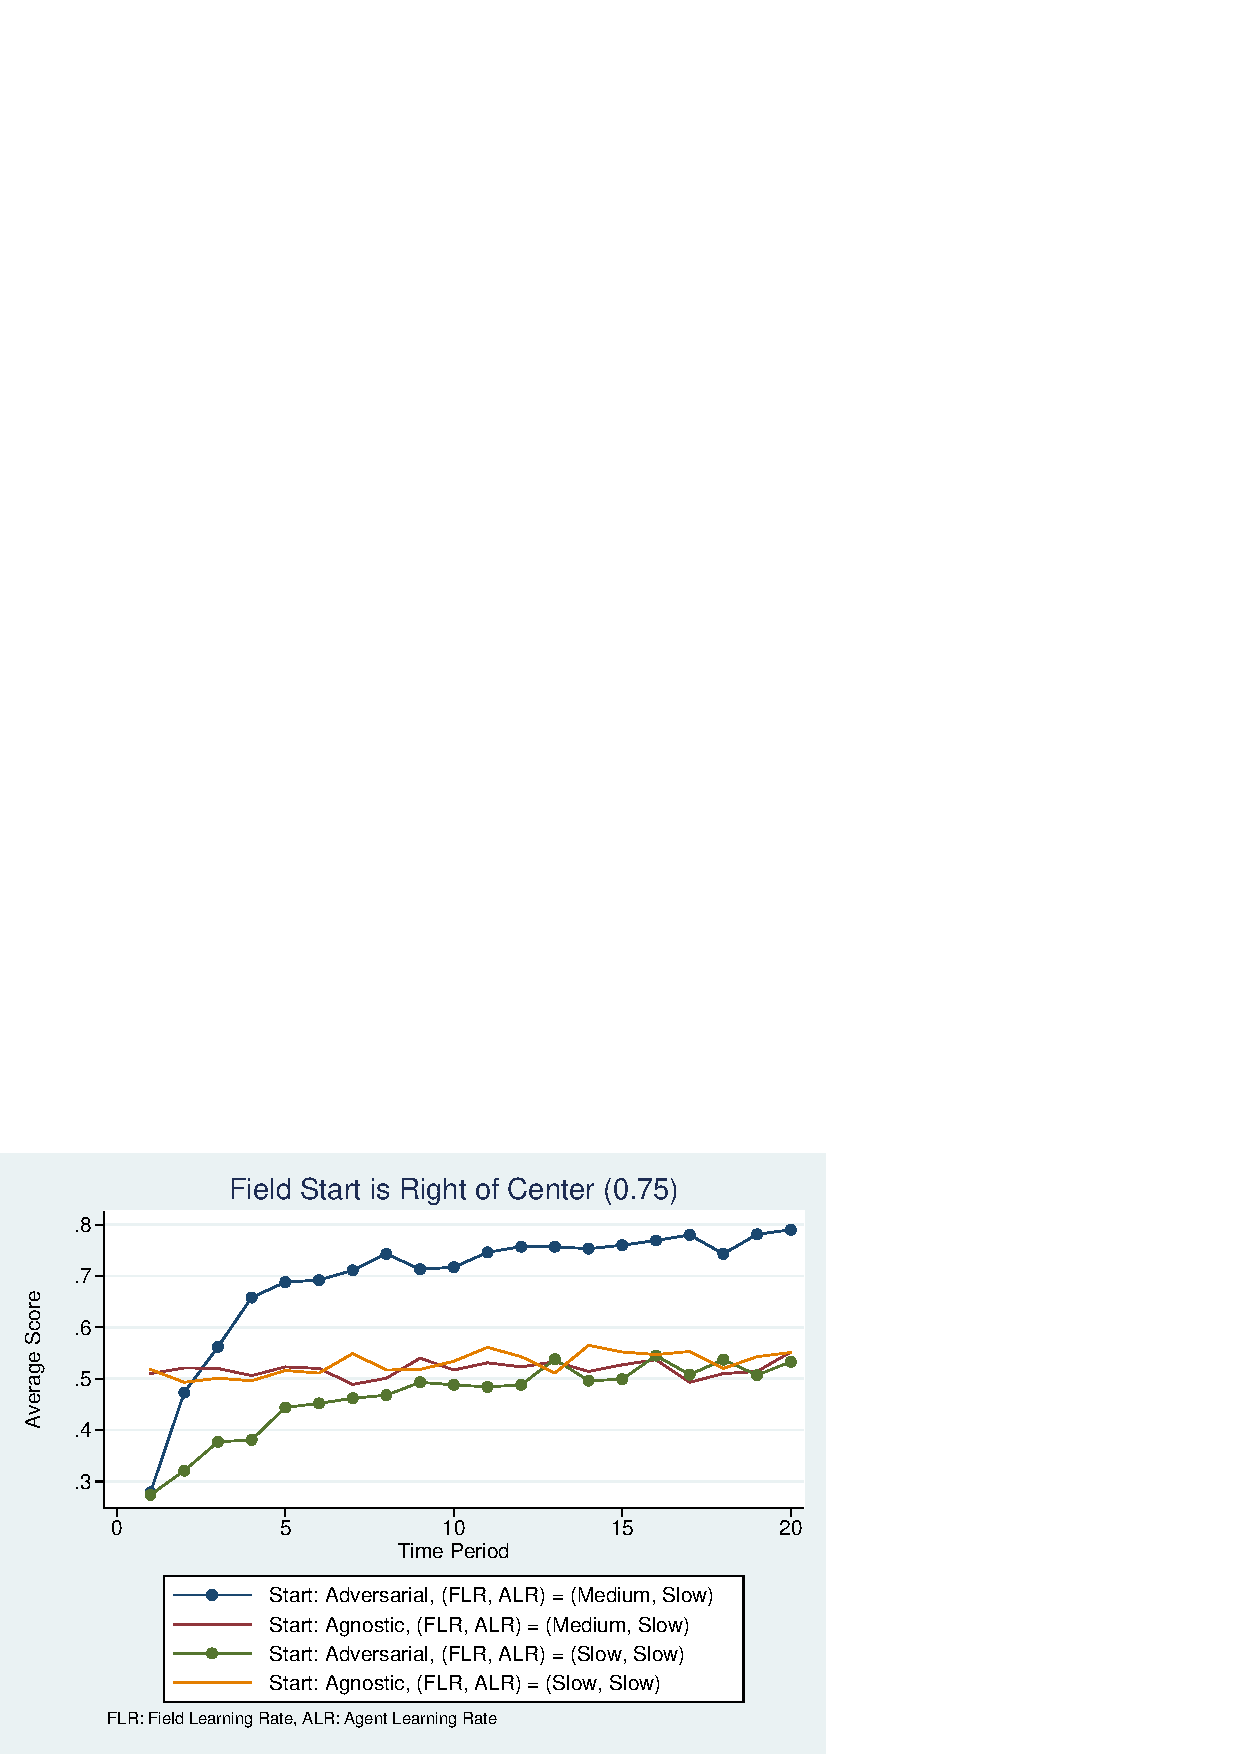
\includegraphics[width=\textwidth]{frcmedium3a}
  \caption{}
  \label{fig:3a}
\end{centering}
\end{figure}

\begin{figure}[h]
\begin{centering}
  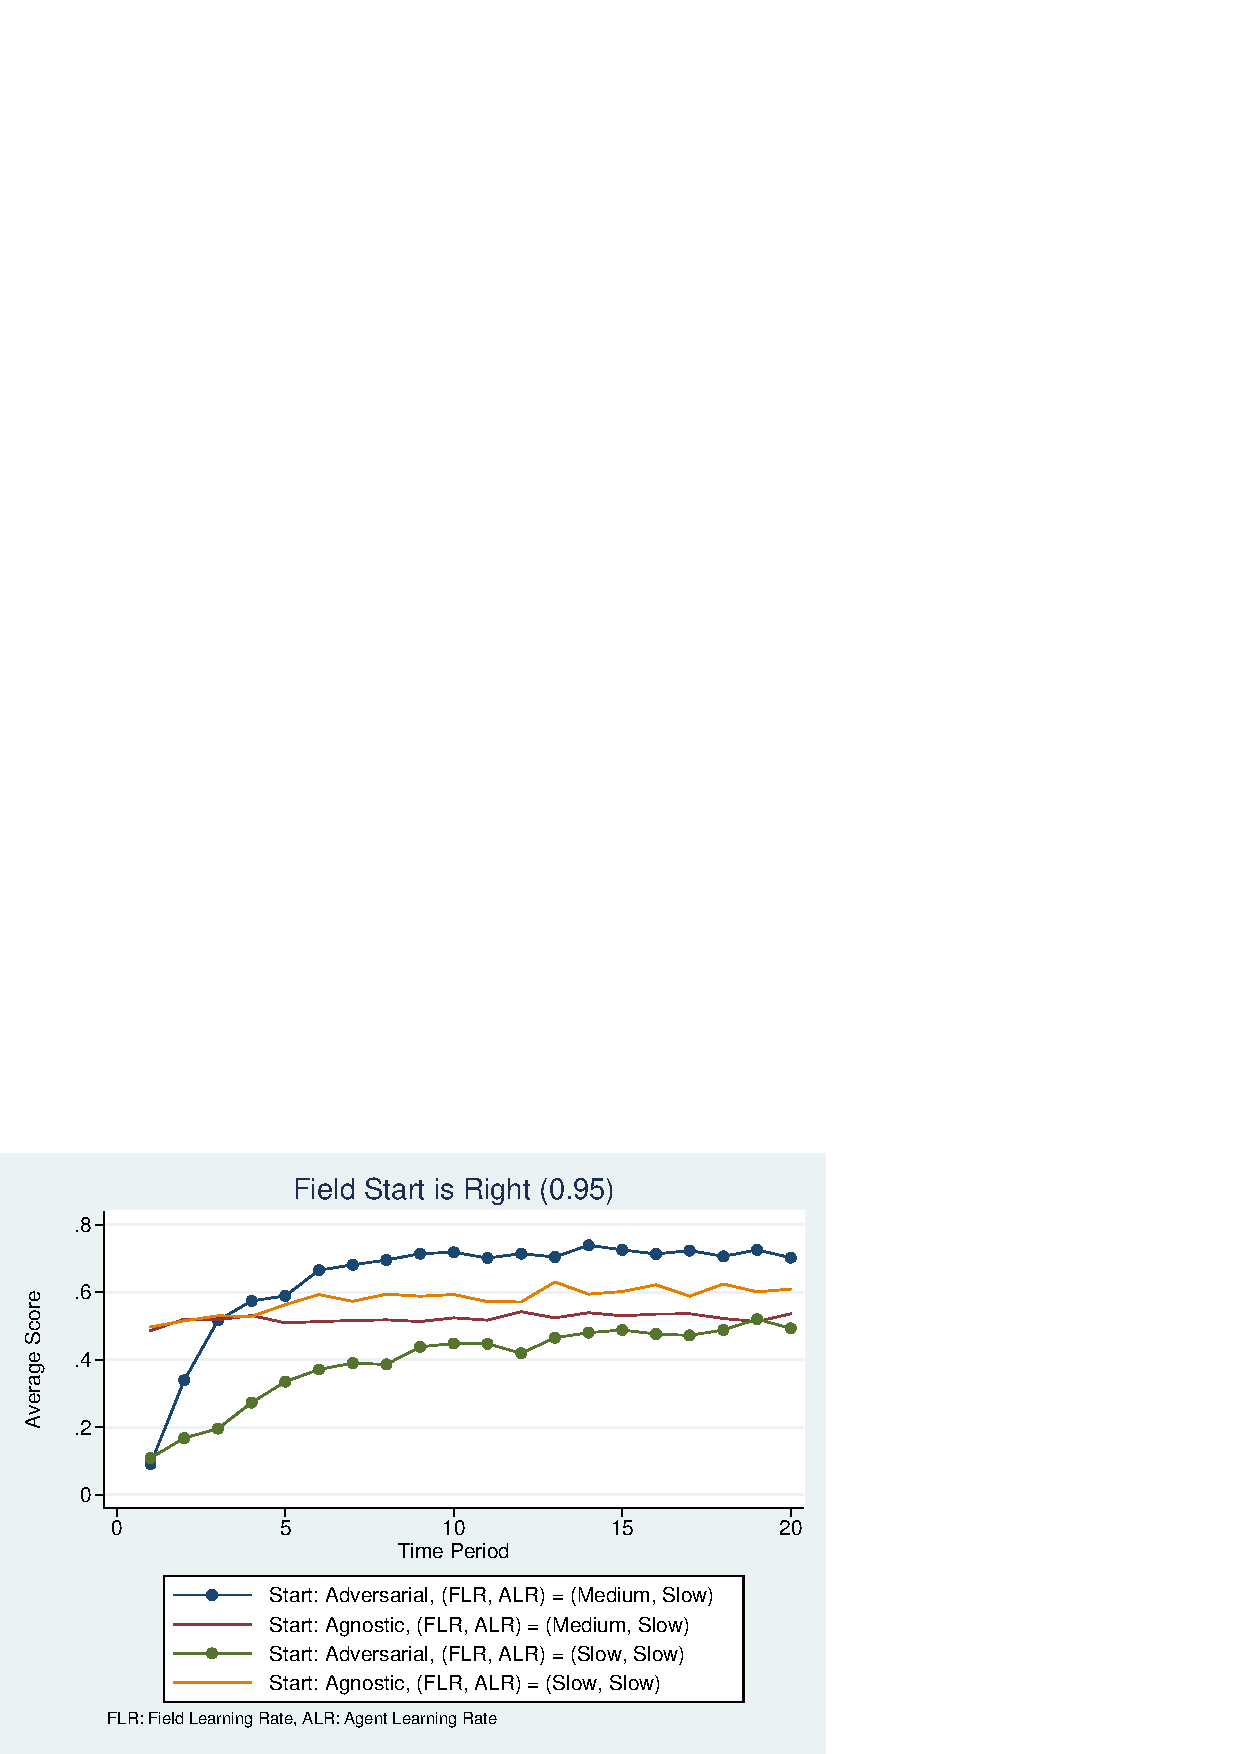
\includegraphics[width=\textwidth]{frcmedium3b}
  \caption{}
  \label{fig:3b}
\end{centering}
\end{figure}

\section{Appropriateness of the Matching Model for Embedded Agency-Institutional Field Interaction}
\noindent Having laid out the formal model and having described the assumptions and classifications made in the previous section, it seems appropriate to now consider if the model described above is a reasonable abstraction of the phenomenon that we wish to theorize upon. We consider this in the current section.\\\\

\noindent We use an example to illustrate our argument. In the arena of international business, the decision making behavior of the MNC subsidiary is considered a classical case for the institutional theory argument. The institutional field of the MNC subsidiary consists of the MNC parent firm, the legal and intellectual property regimes in the host country, and other organizations such as compatriot MNC subsidiaries in the same region, other firms in the supply chain and host country HR attributes. Scholars have demonstrated that such MNC subsidiaries have significant autonomy in decision making due to the varied nature of stakeholders that have to managed in the smooth functioning of the MNC subsidiaries. \\\\
It is therefore reasonable to model the embedded agent (the MNC subsidiary in this case) as one with the three varied positions at the start: Aligned, where the MNC subsidiary's prior preferences are aligned to that of its institutional field (the host government and the MNC parent all want the same thing, say the outsourcing of more IT services to the Indian subsidiary); Agnostic, where it may not be clear to the MNC subsidiary if it should or should not take up a decision, say of say launching a consulting division of the business. A situation like this may arise because the MNC subsidiary sees both advantages and disadvantages from such a move owing to their understanding of the ground situation, while the MNC parent or the government or the workforce at large may be glossing over potential scaling or integration issues; and finally Adversarial, where the MNC subsidiary's initial position is at odds with that of the MNC parent or the larger institutional field. We know of several such examples, including that of the Indian Tobacco Company (ITC) several decades ago. \\\\

\noindent Having addressed the classification of initial preferences for the agent, we now consider the classification proposed for the institutional field. Given that an institutional field is a complex multitude of several organizations, the question that comes up is if the institutional field should be modeled to reflect the complexity of its underlying constituents, or if it should be modeled based on how it is perceived by the embedded agent. Clearly there are advantages and disadvantages with both approaches. We chose the latter approach because of the simplicity. \\\\
In essence, our model assumes that the institutional field's priors are either one where it favors an outcome of 0 with a 0.95 probability (the configuration that we describe as "Right" for the lack of a more meaningful alternative), or one where it favors an outcome of 0 with a 0.75 probability (the configuration that we describe as "Right of Center" in keeping with our Left-Center-Right terminology). Our conception of an institutional field with a right orientation is one that has a strong initial preference for one set of outcomes, and when associated with a slow rate of learning, equivalent to the structuration resembling the iron cage as described in the literature. A "Right" initial orientation with a medium rate of learning and a "Right of Center" initial orientation with a slow rate of learning capture the classic tradeoff between starting position and adaptation capacity. Finally, the "Right of Center" initial orientation coupled with slow learning is one that captures the rather complex pulls and pushes of the various stake holders in the institutional field who are unable to move the field to any strong consensus in any reasonable period of time. Between the four combinations of characterizations for the institutional field,  we have captured the salient aspects of complex interaction as well as coordinated harmony in institutional fields.\\\\

\noindent A question may arise about the appropriateness of the matching mechanism for studying the dynamics of agent-field interactions. Clearly, the payouts are not in perfect alignment or in perfect misalignment in real agent-field interactions in the real world. Second, most agent-field interactions are not settled at every time period, nor is it necessary or appropriate there agents pursue a single objective at a point of time. Indeed, as suggested by \cite{Kostova2008}, it is quite common for agents to engage in decoupling behavior with ceremonial adoption of institutionalized structures along side the pursuit of specific economically efficient practices. We are sympathetic to these concerns, and believe that these must at some stage be incorporated into computational models. However, it seemed overly ambitious to take those up in the initial study, and were hence left out.\\\\

\noindent Finally, it is worth noting two other points. First, that while the embedded agents are allowed three learning rates: slow, medium and fast; institutional fields are allowed only two: slow and medium. This is just an outcome of the complexity assumption,  that highly complex organizational forms may not adapt as quickly as less complex organizational forms. Second, because of our classification of initial position of the agent as one in contrast to that of the field, we did not require to consider data from our experiments where the institutional field's starting orientation was "Left" or "Left of Center". This is so because a field orientation of "Left", and an agent orientation of agnostic would be no different from a field orientation of "Right" and an agent orientation of agnostic. A similar argument could be made for "Left, Adversarial" and being no different from "Right, Adversarial". However we do drop the "Center" orientation of the institutional field as a simplification for the current study. It is conceivable that a "Center" initial orientation and slow learning disposition may capture the highest strain of conflict in the institutional field, but it was left out of this study so as to focus more on the configurations in the middle where the answers to appropriate agent action are not particularly obvious.\\\\

\section{Interpretation of Model Results}
\noindent In order to understand the effect of each change on the outcome, we proceed to understand the effects of field configuration and agent configuration on overall outcome one change at a time. Figure ~\ref{fig:3a} lays out the average score charts for four agent-field combinations while enforcing the field to start in Right of Center (this is the same as saying $p_{0,F}^0 = 0.75$). Figure ~\ref{fig:3a} demonstrates that an adversarial agent with a slow rate of learning ($\phi_A = 0.05$) is likely to get stuck at a peak average performance of around 0.5, whereas one in medium learning rate field is likely to reach a peak average performance of close to 0.8 (This is the comparison of the two dotted lines graphs in blue and green). On the other hand, we notice that agnostic agents do similarly despite changes in the rate of learning of the field F. The interesting result from Figure ~\ref{fig:3a} is that though adversarial agents start off with contradictory preferences to the field, they end up with a higher average score than the agnostic agents who start off with a better alignment (0.5 is more aligned to 0.95 than is 0.05). The logic for this result is that the adversarial agent is actually adapted by the field F due to its relatively higher learning rate. In the case of the adversarial agent in the (Slow, Slow) configuration, the agent was stuck with $p_{t,A}^0$ closer to 0.5 with the field F unable to pull that agent A up quickly enough due to it's slow rate of learning. This (adversarial agent in a (Slow, Slow)) configuration is therefore a good candidate for a change in setting.\\\\



\begin{figure}[h]
\begin{centering}
  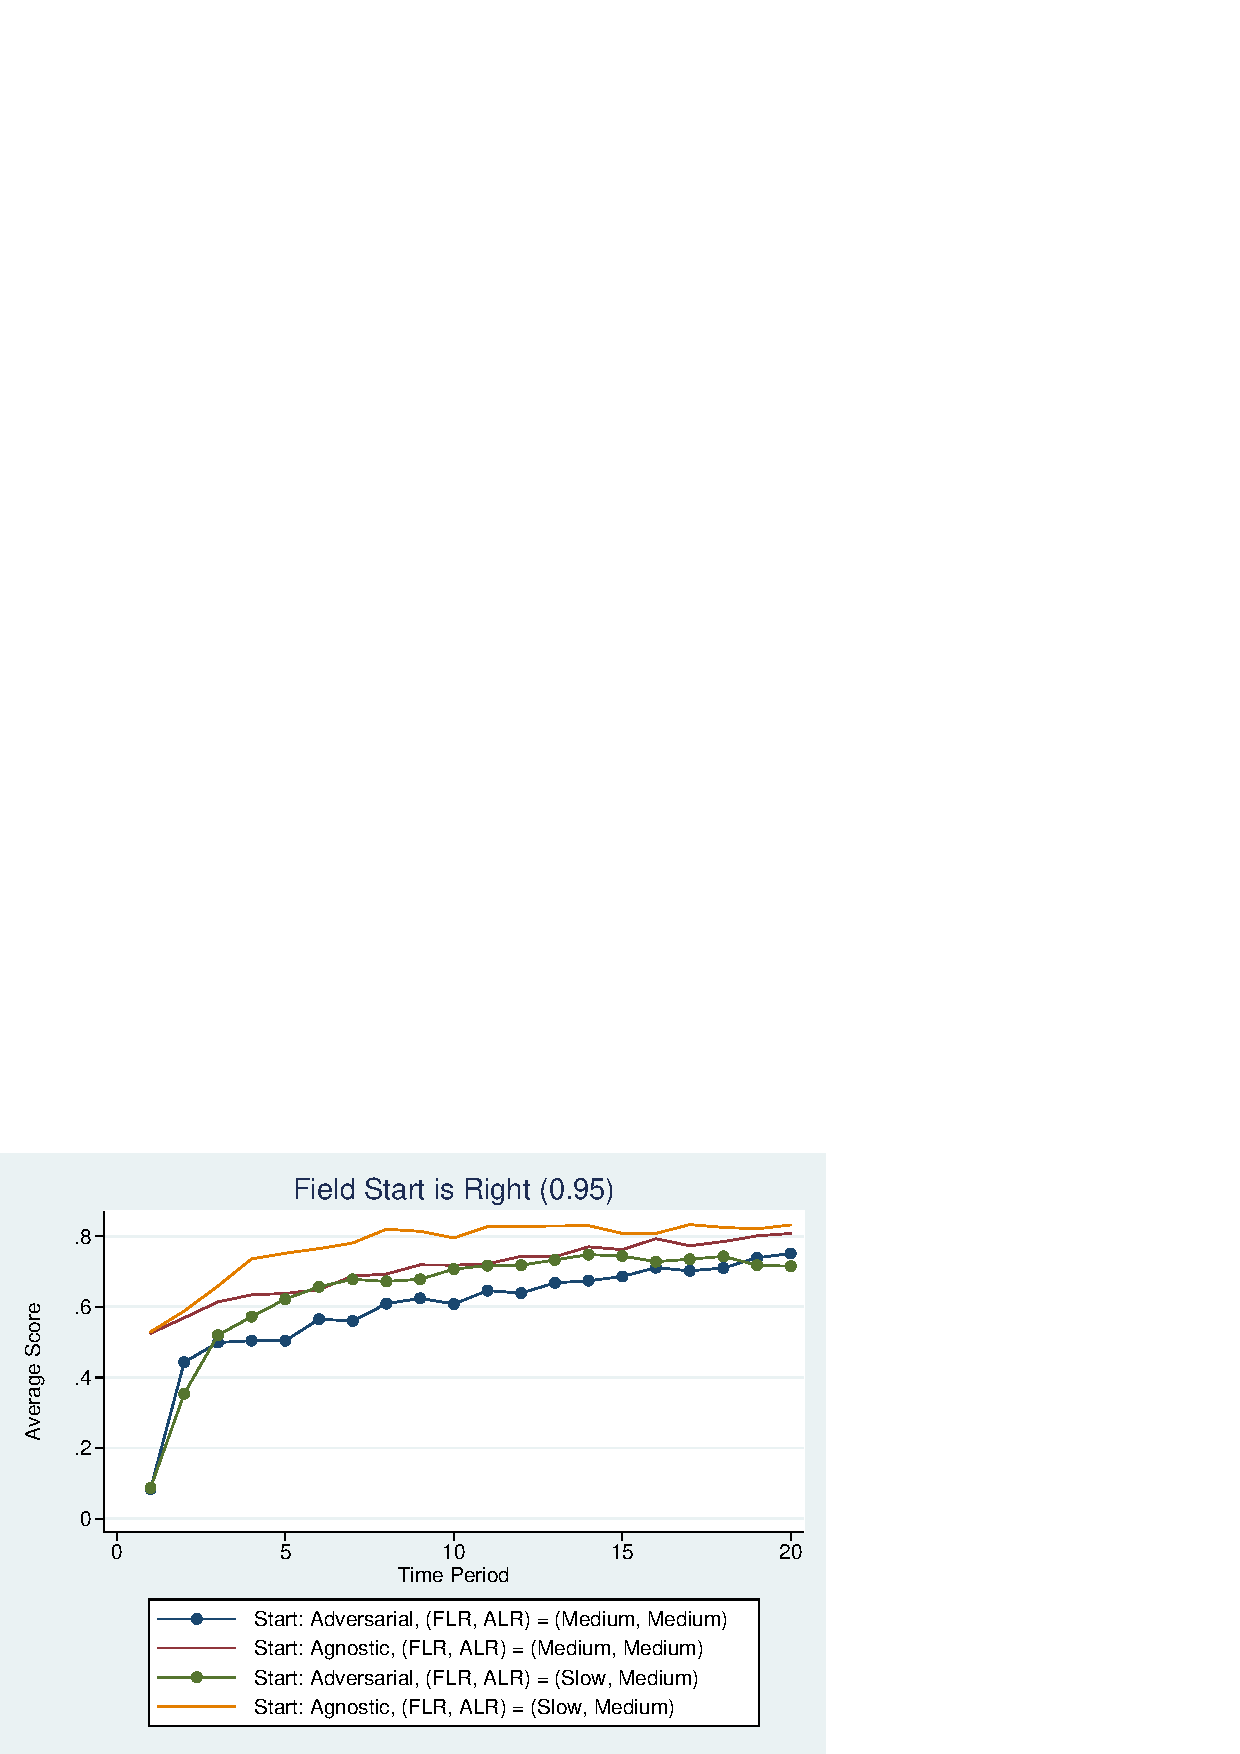
\includegraphics[width=\textwidth]{frcmedium3c}
  \caption{}
  \label{fig:3c}
\end{centering}
\end{figure}

\noindent In moving from Figure ~\ref{fig:3a} to Figure ~\ref{fig:3b}, we shift the initial preference of the institutional field from Right of Center, to Right. This effectively increases the initial divergence in the preferences between agents and the institutional field. We observe that the peak average score for the slow learning adversarial agent is lower as compared to the peak average score of the slow learning adversarial agent in Figure ~\ref{fig:3a}. This result is to be expected because of the increased burden on the institutional field to bridge a wider gap in initial preferences.\\\\

\begin{figure}[h]
\begin{centering}
  \includegraphics[width=\textwidth]{frcmedium3d}
  \caption{}
  \label{fig:3d}
\end{centering}
\end{figure}

\noindent In moving from Figure ~\ref{fig:3b} to Figure ~\ref{fig:3c}, we raise the agent learning rate from slow to medium for all configurations while keeping everything else constant. We observe here that the increased learning rate increases the overall performance in all configurations, but the greatest gains are made in configurations with agnostic agents. The effect that we had observed in Figure ~\ref{fig:3a} and Figure ~\ref{fig:3b} may therefore be confirmed to be due to the differential rate of learning of the agents with respect to the institutional field. Once agents were allowed to increase their rate of learning, the adversarial agents are no longer better than agnostic agents. Indeed, Figure ~\ref{fig:3c} demonstrates that the agnostic agents who begin being neutral to either outcome are able to use their superior learning rates to achieve a higher level of overall performance. This trend is confirmed further in Figure ~\ref{fig:3d} where the learning rates of agents are increased even further to "Fast".\\\\

\begin{figure}[h]
\begin{centering}
  \includegraphics[width=\textwidth]{frcmedium3e}
  \caption{}
  \label{fig:3e}
\end{centering}
\end{figure}

\noindent Our next experiment studies the effect of increasing the initial level of openness of the institutional field while retaining the learning rates of the agents at "Fast". We notice from comparing Figure ~\ref{fig:3e} with Figure ~\ref{fig:3d} that a performance gap opens up between the slow learning institutional field and the medium learning institutional field. This leads us to an interesting insight that increasing the learning rate differential between the institutional field and the agent is useful up to a point, after which a large divergence in learning ability results in a lower level of overall outcome.\\\\
\begin{figure}[h]
\begin{centering}
  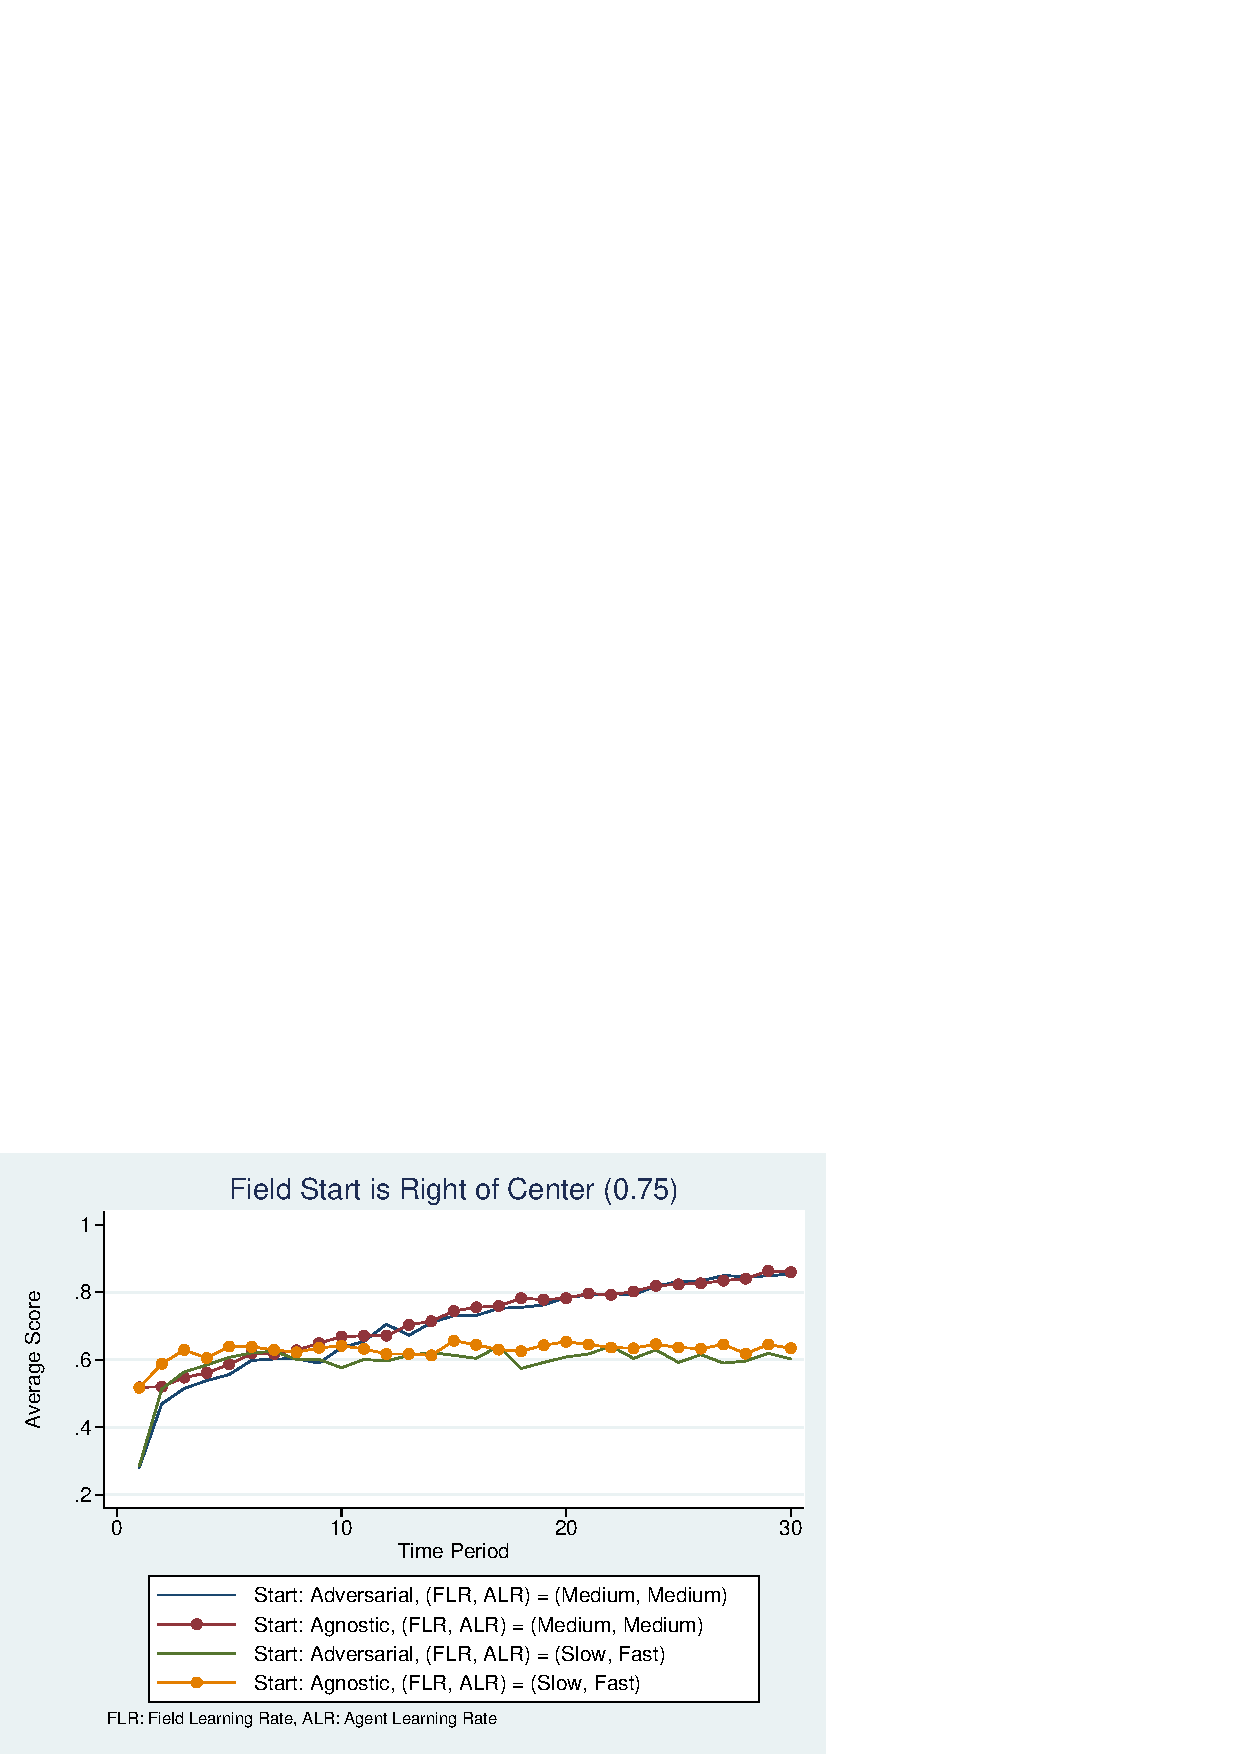
\includegraphics[width=\textwidth]{frcmedium3f}
  \caption{}
  \label{fig:3f}
\end{centering}
\end{figure}

\noindent Figure ~\ref{fig:3f} illustrates the effect of reducing the rate of learning of the fast learning agents to medium, keeping all else the same. We notice that the average overall performance drops as a result. The trends from Figure ~\ref{fig:3d}, Figure ~\ref{fig:3e}, and Figure ~\ref{fig:3f} suggest that the outcomes may initially increase with increased difference in learning abilities and then drop. This trend is confirmed in Figure ~\ref{fig:3g} where we drop the learning rate of one set of agents all the way to slow. Clearly this result is hardly surprising, as one would expect fast learning agents to contribute higher to overall outcomes than slow learning ones.\\\\

\begin{figure}[h]
\begin{centering}
  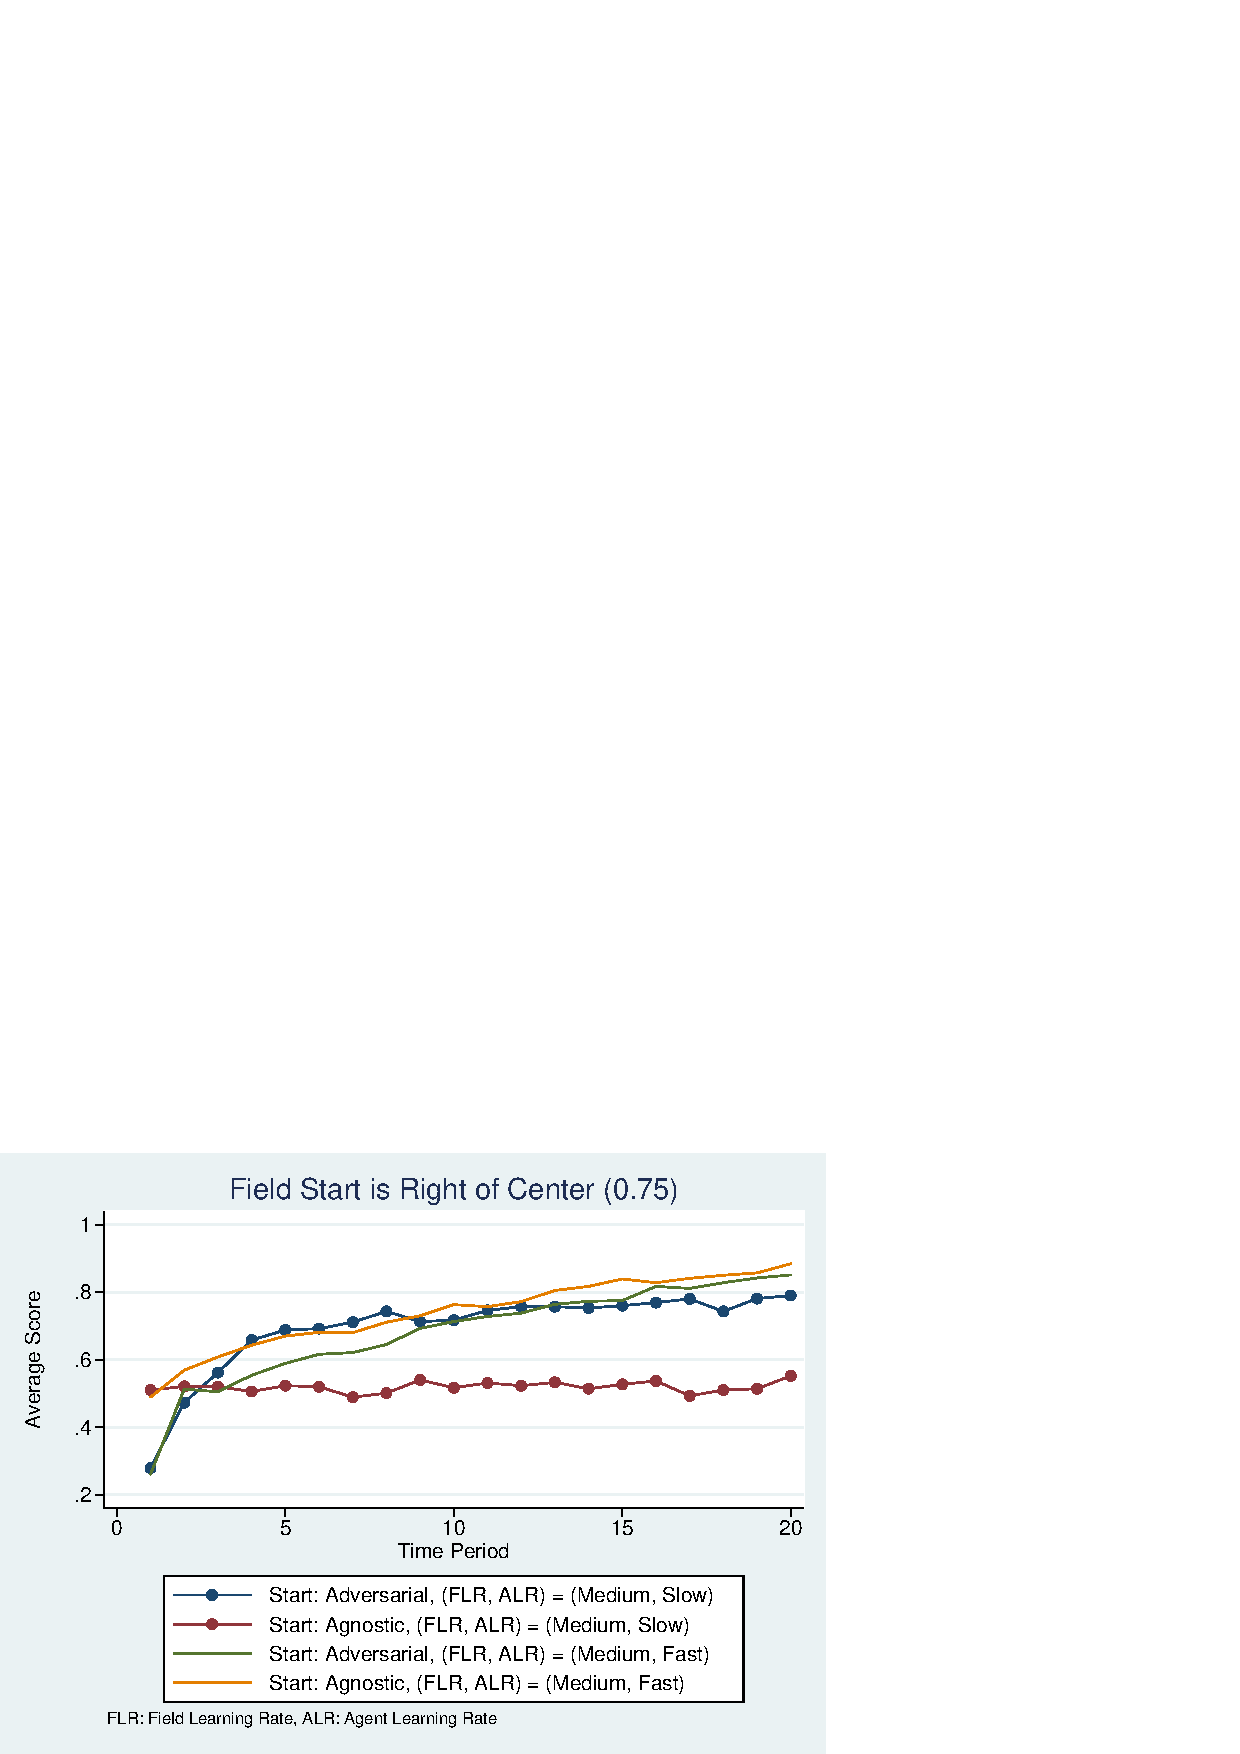
\includegraphics[width=\textwidth]{frcmedium3g}
  \caption{}
  \label{fig:3g}
\end{centering}
\end{figure}

\section{Hypotheses}
\noindent Based on discussions in the previous section, we propose the following hypotheses\\\\
\begin{hypothesis}
{Hypothesis 1a: When the institutional field is open to inluence, slow learning adversarial agents will raise overall performance higher than slow learning agents with a neutral orientation\\}
\end{hypothesis}
\begin{hypothesis}
{Hypothesis 1b: For the same rate of learning for the institutional field, slow learning adversarial agents will raise overall performance less with a larger divergence between the initial preferences between agents and the institutional field\\}
\end{hypothesis}

\begin{hypothesis}
{Hypothesis 2a: For the same initial outcome preferences,  the overall performance score varies curvilinearly with difference in the rates of learning of the agent and the institutional field\\}
\end{hypothesis}
\begin{hypothesis}
{Hypothesis 2b: For the same initial outcome preferences,  the overall performance score drops as the difference in the rates of learning of the agent and the institutional field drops\\}
\end{hypothesis}

\begin{hypothesis}
{Hypothesis 3: An increase in the openness of an institutional field does not raise overall performance when agents have a neutral orientation with a slow rate of learning\\}
\end{hypothesis}

\section{Limitations and Future Work}
\noindent The formal computational modeling approach to theorizing organizational phenomena seems both valuable as well as challenging. While the fine grained control and possibility of step by step changes in experiments allows for a detailed understanding of micro phenomena, the very flexibility also creates a problem of plenty. However, with the appropriate priorities this should be a good problem to have.\\\\
The big question relevant for institutional theory applications is how to model the institutional field. A potential alternative to the current simplifying assumption coming from an agent view of the institutional field is to develop independent models of the institutional field with its associated components, and to possibly use the outcomes from such models to inform our model of the institutional field. Clearly, there is much further to go on this question before anything may be applied to the practice of research.\\\\
We would like to highlight three specific points that can be developed upon in future work. First, it seems unrealistic to assume that either agents or institutional fields have a constant rate of learning for all time. An interesting experiment would be to allow for both phases of inspiration (a higher rate of learning) and phases of boredom (lower or counter productive learning) while maintaining some average learning rate. Second, decoupling seems to an important phenomenon in practice that is has also been hard to formalize using traditional empirical methods. It seems like modeling embedded agency with decoupling could lead to very interesting opportunities to theorize organizational phenomena. Finally, the inclusion of decoupling could possibly suggest relooking the assumption of the matching game. As was noted earlier in the article, agents and fields are probably updating their priors less often, and with less perfect information that has been assumed in the current model. Allowing for some flexibility there could help us capture the nuances of the agent field interaction in greater depth.\\\\

\section{Acknowledgements}
I am heavily indebted to Abhoy Ojha for having set the bar for this paper high. I am indeed the biggest beneficiary of the expectation of as full a paper as possible. My ability to do this work was also contributed to by Sai Yayavaram, who introduced me in June 2015 to the wonderful world of computational modeling, and to Phanish Puranam who helped me with thinking about simple agent based models for modeling organizational phenomena. All mistakes made here are completely mine.

\bibliography{/Users/aiyenggar/OneDrive/code/bibliography/ae,/Users/aiyenggar/OneDrive/code/bibliography/fj,/Users/aiyenggar/OneDrive/code/bibliography/ko,/Users/aiyenggar/OneDrive/code/bibliography/pt,/Users/aiyenggar/OneDrive/code/bibliography/uz} 
\bibliographystyle{apalike}

\appendix

\section{Simulation Code}
\lstinputlisting{ot-term-paper-images/matchingEmbeddedAgency.py}

\section{Analysis Code}
\lstinputlisting{ot-term-paper-images/embeddedAgent.do}

\end{document}
